\documentclass{article}
\usepackage[utf8]{inputenc}

\title{Assignment 4: Local Search}
\author{Brian Jacobel}
\date{Artificial Intelligence, Fall 2013}

\usepackage{natbib}
\usepackage{graphicx}
\usepackage[margin=1in]{geometry}
\usepackage{setspace}
\usepackage{indentfirst}

\begin{document}

\maketitle

\begin{doublespace}

\section{Introduction}
In this lab, I implemented the local search algorithm using the \textsc{min-conflicts} heuristic in a program designed to efficiently solve the ``$n$-queens" problem. This constraint satisfaction problem describes the task of placing $n$ queens on an $n$-by-$n$ chessboard, and iteratively arranging them so that no queen is in a position of being able to capture another queen within a single move. In this problem, there are $6n-2$ constraints: $n$ constraints specify that each column may have only one queen, $n$ constraints specify the same for each row, $2n-1$ constraints specify that there may be only one queen in each upwards-sloping diagonal, and $2n-1$ constraints say the same for each downwards-sloping diagonal. The column constraints can be thought of as ``freebies" -- that is, queens can be obviously distributed at the start such that each is in a separate column, and this can be maintained throughout the problem easily. Thus, the variables that form the search space for this problem are simply the row locations for each queen.

\section{Testing methodology}
My algorithm is contained in the Python module \texttt{nqueens.py}, which can be run interactively via the command line if the user wishes. For testing, this code is imported into the script \texttt{test.py}, which runs the code a number of times and averages statistics. For each run of \texttt{test.py}, the $n$-queens problem is solved ten times each with with $n$ starting at 5 and incrementing by 5 up to a maximum of 60. At each value of $n$, the average run time for the problem to be solved and the average number of moves required to find that solution is displayed. If one of the ten trials should fail, only successful trials are included in these values. However, in my tests, my program seldom failed to find a solution to the problem for a value of $n$ less than 100. 

I ran \texttt{test.py} six times: one for each of the variants of the algorithms explored in the assignment. In the upcoming section, I will display and discuss the differences in generated results between these algorithm variants.

As a point of comparison between my results and others', my testing was done on a fairly old Intel Xeon E5620 machine (a 2010 Mac Pro) with eight cores clocked to 2.40GHz. This CPU is somewhere in the neighborhood of 60\% as fast as the newer i7-2600 CPUs in Searles 224's iMacs, according to benchmarks I found online. 

\section{Algorithm Variants}
\subsection{Basic implementation}
For the basic local search algorithm with \textsc{min-conflicts} as a heuristic, I obtained the results shown in \textit{Fig. 1}. The algorithm's performance as measured by moves shows, after a large initial jump, a roughly linear growth from 60 to 120. On the other hand, the algorithm's performance as measured by time shows an exponential increase as the size of the problem increases. A trendline plotted through these data points conformed to the equation $4.17x^{3.23}$, meaning the running time of this algorithm is roughly bound by $O(n) = 4x^4$. \\

\begin{figure}[ht!]
\centering
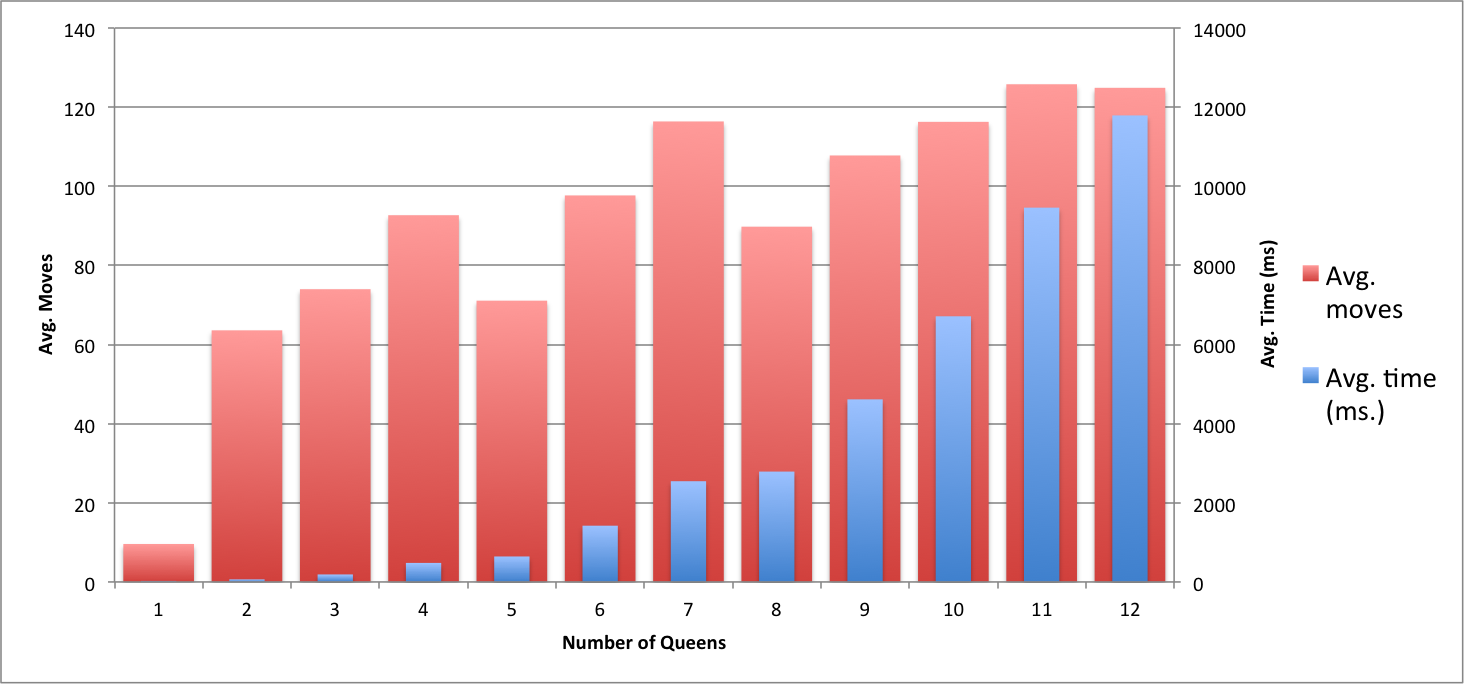
\includegraphics[width=6.5in]{./base.png}
\caption{Performance of the basic local search algorithm, in moves and time.}
\end{figure}

\newpage

\subsection{Greedy implementation}
The results of the greedy variant of this algorithm, where the queen to move rather than being picked randomly is the queen with the greatest number of conflicts, are shown in \textit{Fig. 2}. The data conform to the same general patterns shown above: a linear increase in average moves performed an a power increase in the running time.

\begin{figure}[ht!]
\centering
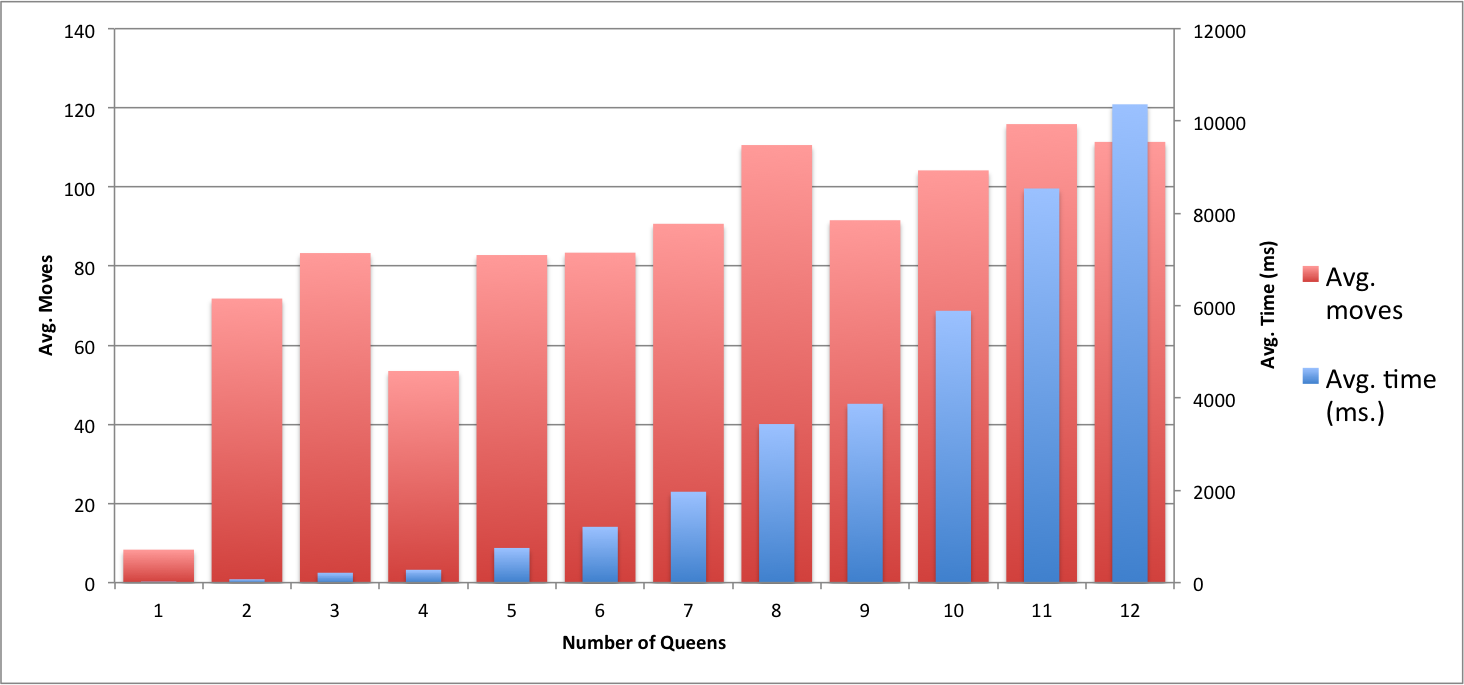
\includegraphics[width=6.5in]{./greedy.png}
\caption{Performance of the greedy variant of the local search algorithm, in moves and time.}
\end{figure}


\subsection{Random implementation}
In this algorithm variant, an unsatisfying queen is picked in the same way as in the basic algorithm. At this point, with some probability, instead of using the standard \textsc{min-conflicts} heuristic to find a new location for this queen, this modified algorithm instead randomly picks a location in the queen's column to place it. In my trials, I found the probability 20\% a good portion of the time to move randomly rather than heuristically; percentages higher than this resulted in the problem not being solved for a significant portion of the tests run. At 20\% random movement, the constraints failed to be satisfied after 500 tries once with 35 queens, three times with 55 queens and once with 60 queens. This represents an overall failure rate of 4.16\%, as opposed to the base algorithm and the previous variant's failure rate of 0\%. Results from this variant are shown in \textit{Fig. 3}.

Of particular note here is that both the number of moves and the time are significantly larger than in the previous two implementations of the algorithm. Comparison between the variants will be discussed further in the next section.

\begin{figure}[ht!]
\centering
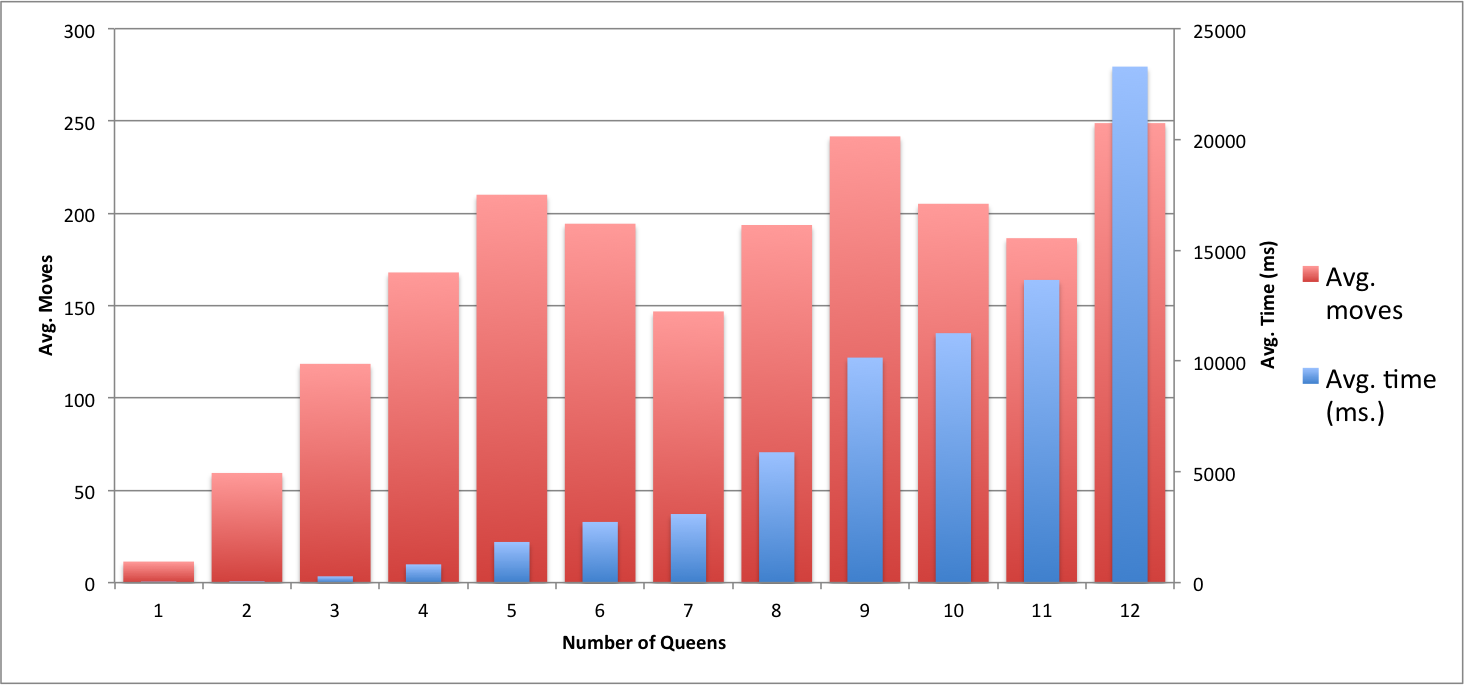
\includegraphics[width=6.5in]{./random.png}
\caption{Performance of the local search algorithm with enhanced randomness, in moves and time.}
\end{figure}

\subsection{Comparison of above variants}
As can be seen in \textit{Fig. 4}, the data for all three algorithm implementations considered thus far follow the same basic pattern: an average number of moves to the solution that is bounded linearly, and an average time to the solution that is bounded by a power function (likely $x^4$). However, it is obvious that one of the variants was not an improvement. At its worst ($n=45$), search with increased randomness takes more than 2.6 times as long to reach an answer as greedy search. This, combined with the fact that search with randomness was causing the failure of about 4\% of test cases (as opposed to no test cases failed in the other two variants) lead us to discard increasing randomness as an option for improving local search for this problem. This is not surprising, as this variant essentially says to do the same thing as the base algorithm would have you do, except 20\% of the time, when you should take an action that is $\frac{n-1}{n}$\% likely to be the wrong one. Randomness may help avoid plateaus and ``getting stuck," but that wasn't a problem that we were having in solving $n$-queens (partly because of the strength of our heuristic).

Of the two remaining algorithm variants, greedy search appears to have the slight advantage in running time (and also moves, which I have not graphed because it is less interesting). In the three cases I will discuss next, I have used the greedier variant of local search as a base for improvement.

\begin{figure}[ht!]
\centering
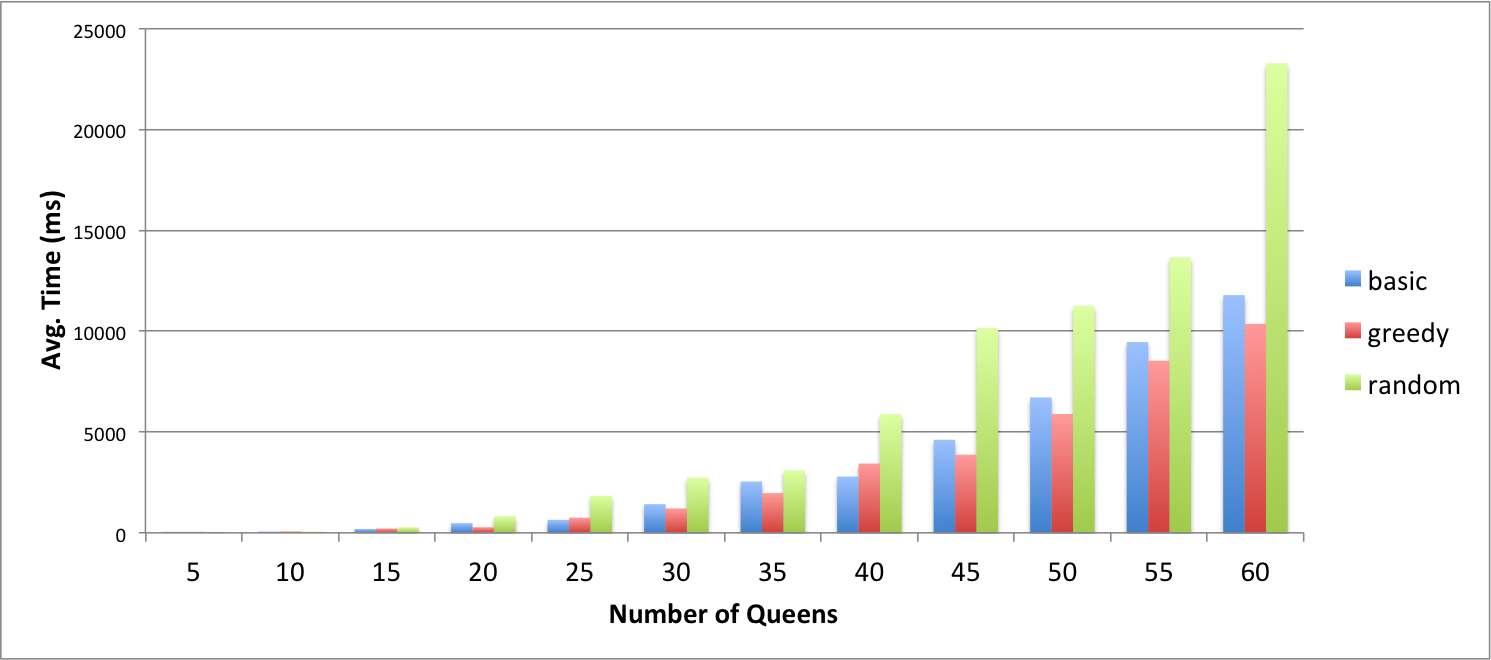
\includegraphics[width=6.5in]{./compare1-3.png}
\caption{Comparison of the first three local search algorithm variants. Search with enhanced randomness is clearly inferior.}
\end{figure}

\section{Further variation}
\subsection{Smarter initial placement}


\subsection{With restarts}

\subsection{Random movements}

\section{Large values}
My implementation of the \textsc{min-conflicts} algorithm successfully solved the $n$-queens problem for an $n$ of up to 350. Here are the n-values, moves and run times for various large values of n I tried. All tests below were done with the initial, unmodified implementation of the algorithm. Because of the times involved in obtaining the results, each was only run once.

I was slightly disappointed that my implementation of the algorithm could not get anywhere near solving even 1,000 queens in a reasonable amount of time. I do not know if this was a realistic expectation. I have declined to graph these values because of their uneven distribution, incompleteness, and lack of multiple trials to back them up -- a graph would not reveal anything significant other than that this problem gets quite hard to solve with size.\\

\begin{center}
\begin{tabular}{|l | l | l|}
\hline
	n-value & moves to solution & time to solution(sec) \\ \hline
	25 & 28 & 2.456 \\ \hline
	50 & 118 & 6.715 \\ \hline
	75 & 121 & 20.935 \\ \hline
	100 & 188 & 74.017 \\ \hline
	150 & 224 & 281.348 \\ \hline
	200 & 295 & 850.566 \\ \hline
	250 & 298 & 1637.862 \\ \hline
	350 & 407 & 8119.451 (2.255 hours) \\ \hline
	500 & N/A (hit max with 26 conflicts unfixed) & N/A \\ \hline
	1000 & never finished & More than 18 hours \\ \hline
	1000000 & never finished & More than 18 hours \\
\hline
\end{tabular}
\end{center}

\section{Conclusion}




\end{doublespace}

\end{document}



